% -------------------------------------------------------------------
% A simple LaTeX book template
% -------------------------------------------------------------------
\documentclass{lifmanual}
\usepackage{import}

% Generate an index
\makeindex

% ---------------------------------------
% The gitbook-pandoc script will generate a file
% called pandoc.inc.tex, which contains many declarations
% required to compile the book.
% ---------------------------------------
% Here we use a frozen version of pandoc.inc.tex, as we made a few
% modifications to the Pandoc-generated file
\input{pandoc.inc.freeze.tex}

% ---------------------------------------
% Title and author
% ---------------------------------------
\title{Event Stream Processing with BeepBeep}
\author{Sylvain Hallé}
\hypersetup{
  pdftitle = {Event Stream Processing with BeepBeep},
  pdfauthor = {Sylvain Hallé}
}
\usepackage{multicol}
\usepackage{newunicodechar}
\DeclareUnicodeCharacter{2693}{\ding{46}}

\begin{document}
\frontmatter
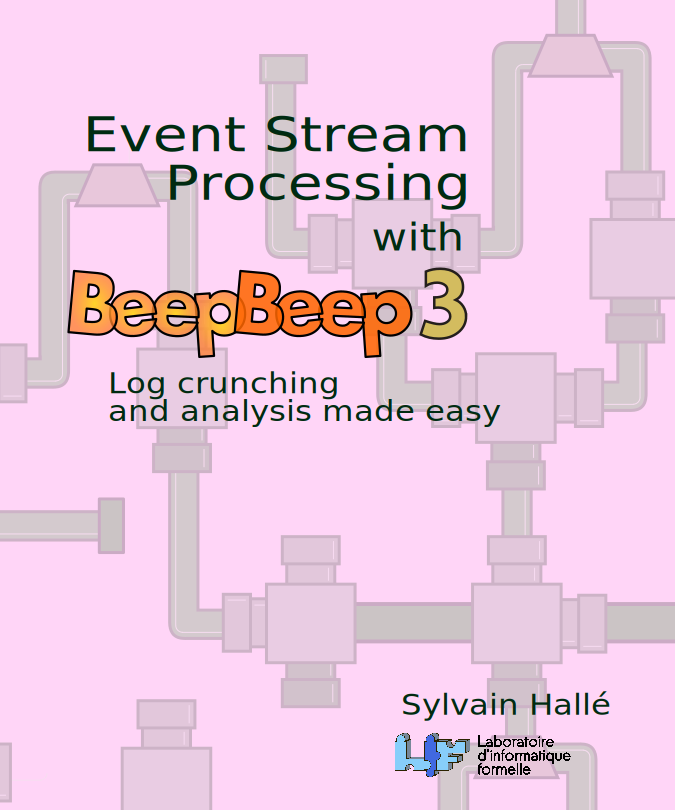
\includepdf[width=7.5in,height=9in]{Cover.pdf}
\newpage

%% 2nd cover
\thispagestyle{empty}
\pagestyle{empty}
\rule{0in}{6in}
\noindent
\includegraphics[width=1in]{by-nc-nd}\\
{\sf\small
\noindent
This work is licensed under the Creative Commons Attribution-NonCommercial-NoDerivatives 4.0 International License. To view a copy of this license, visit \url{http://creativecommons.org/licenses/by-nc-nd/4.0/}.\\

\noindent
\rule{0in}{8pt}
\noindent
Book version: L1.0---March 15, 2018}


\tableofcontents
\newpage

\mainmatter
\thispagestyle{fancy}
\pagestyle{fancy}
\subimport*{chapters/}{body}

\printindex

\end{document}
%% :wrap=soft: